Building a toy model for derivation production jobs offers a simplified framework to effectively simulate and analyze the behavior of real and Monte Carlo (MC) data.
A toy model collection of data can mimic commonalities in both data and MC by filling in branches with a mixture of position coordinate information, momenta, or other details about the detector.  

Integers that are repeated can be easier to compress than floating-point numbers of increased precision, so adjusting the ratio of integers to floats creates a mixture which can yield compression ratios closer to real and MC data.  
Replicating this mixture in a branch give us an effective model that resembles how current derivation jobs act on real and MC simulated data. 
These toy model mixtures provide an avenue to test opportunities for optimizing the memory and storage demands of the GRID by first looking at limiting basket sizes and their effects on compression of branches. 


\section{Toy Model Compression}

\subsection{Random Float Branches} \label{sec:toy_compression_random_float_branches}
There were a number of iterations to the toy model, but the first was constructed by filling a TTree with branches that each have vectors with varying number of random floats to write and read.
Vectors are used in this toy model, as opposed to arrays, because vectors are dynamically allocated and deallocated, which allows for more flexibility when synthesizing AODs. 
This original model had four distinct branches, each with a set number of events (\verb|N=1000|), and each event having a number of entries, vectors with 1, 10, 100, and 1000 floats each.
The script can be compiled with \verb|gcc| or \verb|g++| and it requires all of the dependencies that come with ROOT. 
Alternatively, the script can be run directly within ROOT.

The following function \verb|VectorTree()| is the main function in this code.
What is needed first is an output file, which will be called \verb|VectorTreeFile.root|, and the name of the tree can simply be \verb|myTree|.
% \begin{lstlisting}[language=C]
%   void VectorTree() {
%     std::unique_ptr<TFile> myFile =
%     std::make_unique<TFile>("VectorTreeFile.root", "RECREATE");
%     TTree *tree = new TTree("myTree", "myTree");
%     ...
%   }
% \end{lstlisting}
The toy model starts variable initialization with the total number of events in the branch, i.e. the number of times a branch is filled with the specified numbers per vectors, \verb|N|. 
Additionally the branches have a number of floats per vector, this size will need to be defined as \verb|size_vec_0|, \verb|size_vec_1|, etc.  
The actual vectors that are being stored into each branch need to be defined as well as the temporary placeholder variable for our randomized floats, \verb|vec_tenX| and \verb|float_X|, respectively. 
\begin{lstlisting}[language=C]  
  void VectorTree() {
    ...
    const int N = 1e4; // N = 10000, number of events
    // Set size of vectors with 10^# of random floats
    int size_vec_0 = 1;
    int size_vec_1 = 10;
    int size_vec_2 = 100;
    int size_vec_3 = 1000;

    // vectors
    std::vector<float> vec_ten0; // 10^0 = 1 entry
    std::vector<float> vec_ten1; // 10^1 = 10 entries
    std::vector<float> vec_ten2; // 10^2 = 100 entries
    std::vector<float> vec_ten3; // 10^3 = 1000 entries

    // variables
    float float_0;
    float float_1;
    float float_2;
    float float_3;
    ...
  }
\end{lstlisting}

From here, branches are initialized so each one knows where its vector pair resides in memory.
\begin{lstlisting}[language=C]  
  void VectorTree() {
    ...
    // Initializing branches
    std::cout << "creating branches" << std::endl;
    tree->Branch("branch_of_vectors_size_one", &vec_ten0);
    tree->Branch("branch_of_vectors_size_ten", &vec_ten1);
    tree->Branch("branch_of_vectors_size_hundred", &vec_ten2);
    tree->Branch("branch_of_vectors_size_thousand", &vec_ten3);
    ...
  }
\end{lstlisting}

One extra step taken during this phase of testing is the disabling of \verb|AutoFlush|. 
\begin{lstlisting}
  void VectorTree() {
    ...
    tree->SetAutoFlush(0);
    ...
\end{lstlisting}
Disabling \verb|AutoFlush| allows for more consistent compression across the various sizes of branch baskets. 
If \verb|AutoFlush| were enabled, then across the various branch types, as in \ref{fig:toymodel_compF_rndm_vectors}, ROOT would decide when to compress each branch basket preventing a consistent compression configuration for the toy model.  
The derivation production jobs tested in Chapter $\ref{chap:DAODProd}$ were tested with \verb|AutoFlush| enabled because those tests are focused on memory and disk usage as opposed to mimicing real or MC data, which they are already using.
Following branch initialization comes the event loop where data is generated and emplaced into vectors.

\begin{lstlisting}[language=C]  
  void VectorTree() {
    ...
    // Events Loop
    std::cout << "generating events..." << std::endl;
    for (int j = 0; j < N; j++) {
        // Clearing entries from previous iteration
        vec_ten0.clear();
        vec_ten1.clear();
        vec_ten2.clear();
        vec_ten3.clear();

        // Generating vector elements, filling vectors
        // Fill vec_ten0 
        // Contents of the vector:
        //    {float_0}
        //    Only one float of random value
        float_0 = gRandom->Rndm() * 10; // Create random float value
        vec_ten0.emplace_back(float_0); // Emplace float into vector
        
        // Fill vec_ten1
        // Contents of the vector:
        //    {float_1_0, ... , float_1_10}
        //    Ten floats, each float is random
        for (int n = 0, n < size_vec_1; n++) {
            float_1 = gRandom->Rndm() * 10;
            vec_ten1.emplace_back(float_1);
        }

        // Do the same with vec_ten2 and vec_ten3, except for 
        //     vectors with size 100 and 1000 respectively. 
        
        // After all branches are filled, fill the TTree with 
        //     new branches
        tree->Fill();
    }
    // Saving tree and file
    tree->Write();
    ...
  }
\end{lstlisting}
Once the branches were filled, ROOT then will loop over each of the branches in the TTree and at regular intervals will remove the baskets from memory, compress, and write the baskets to disk (flushed).

As illustrated, the \verb|TTree| is written to the file which allows for the last steps within this script. 

\begin{lstlisting}[language=C]  
  void VectorTree() {
    ...

    // Look in the tree
    tree->Scan();
    tree->Print();

    myFile->Save();
    myFile->Close();
  }

  int main() {
    VectorTree();
    return 0;
  } 
\end{lstlisting}

Upon reading back the ROOT file, the user can view the original size of the file (Total-file-size), the compressed file size (File-size), the ratio between Total-file-size and File-size (Compression Factor), the number of baskets per branch, the basket size, and other information. 
Filling vectors with entirely random values was believed to yield compression ratios close to real data, but the results in Figure \ref{fig:toymodel_compF_rndm_vectors} show changes needed to be made to bring the branches closer to a compression ratio of $\mathcal{O}(5)$.\footnote{This compression factor comes as the average branch compression factor post-derivation job, which is discussed in Section \ref{section: ATLASIO_Derivation}} 
It is evident that branches containing vectors with purely random floats are more difficult to compress due to the high level of randomization.

\begin{figure}[h]
    \centering
    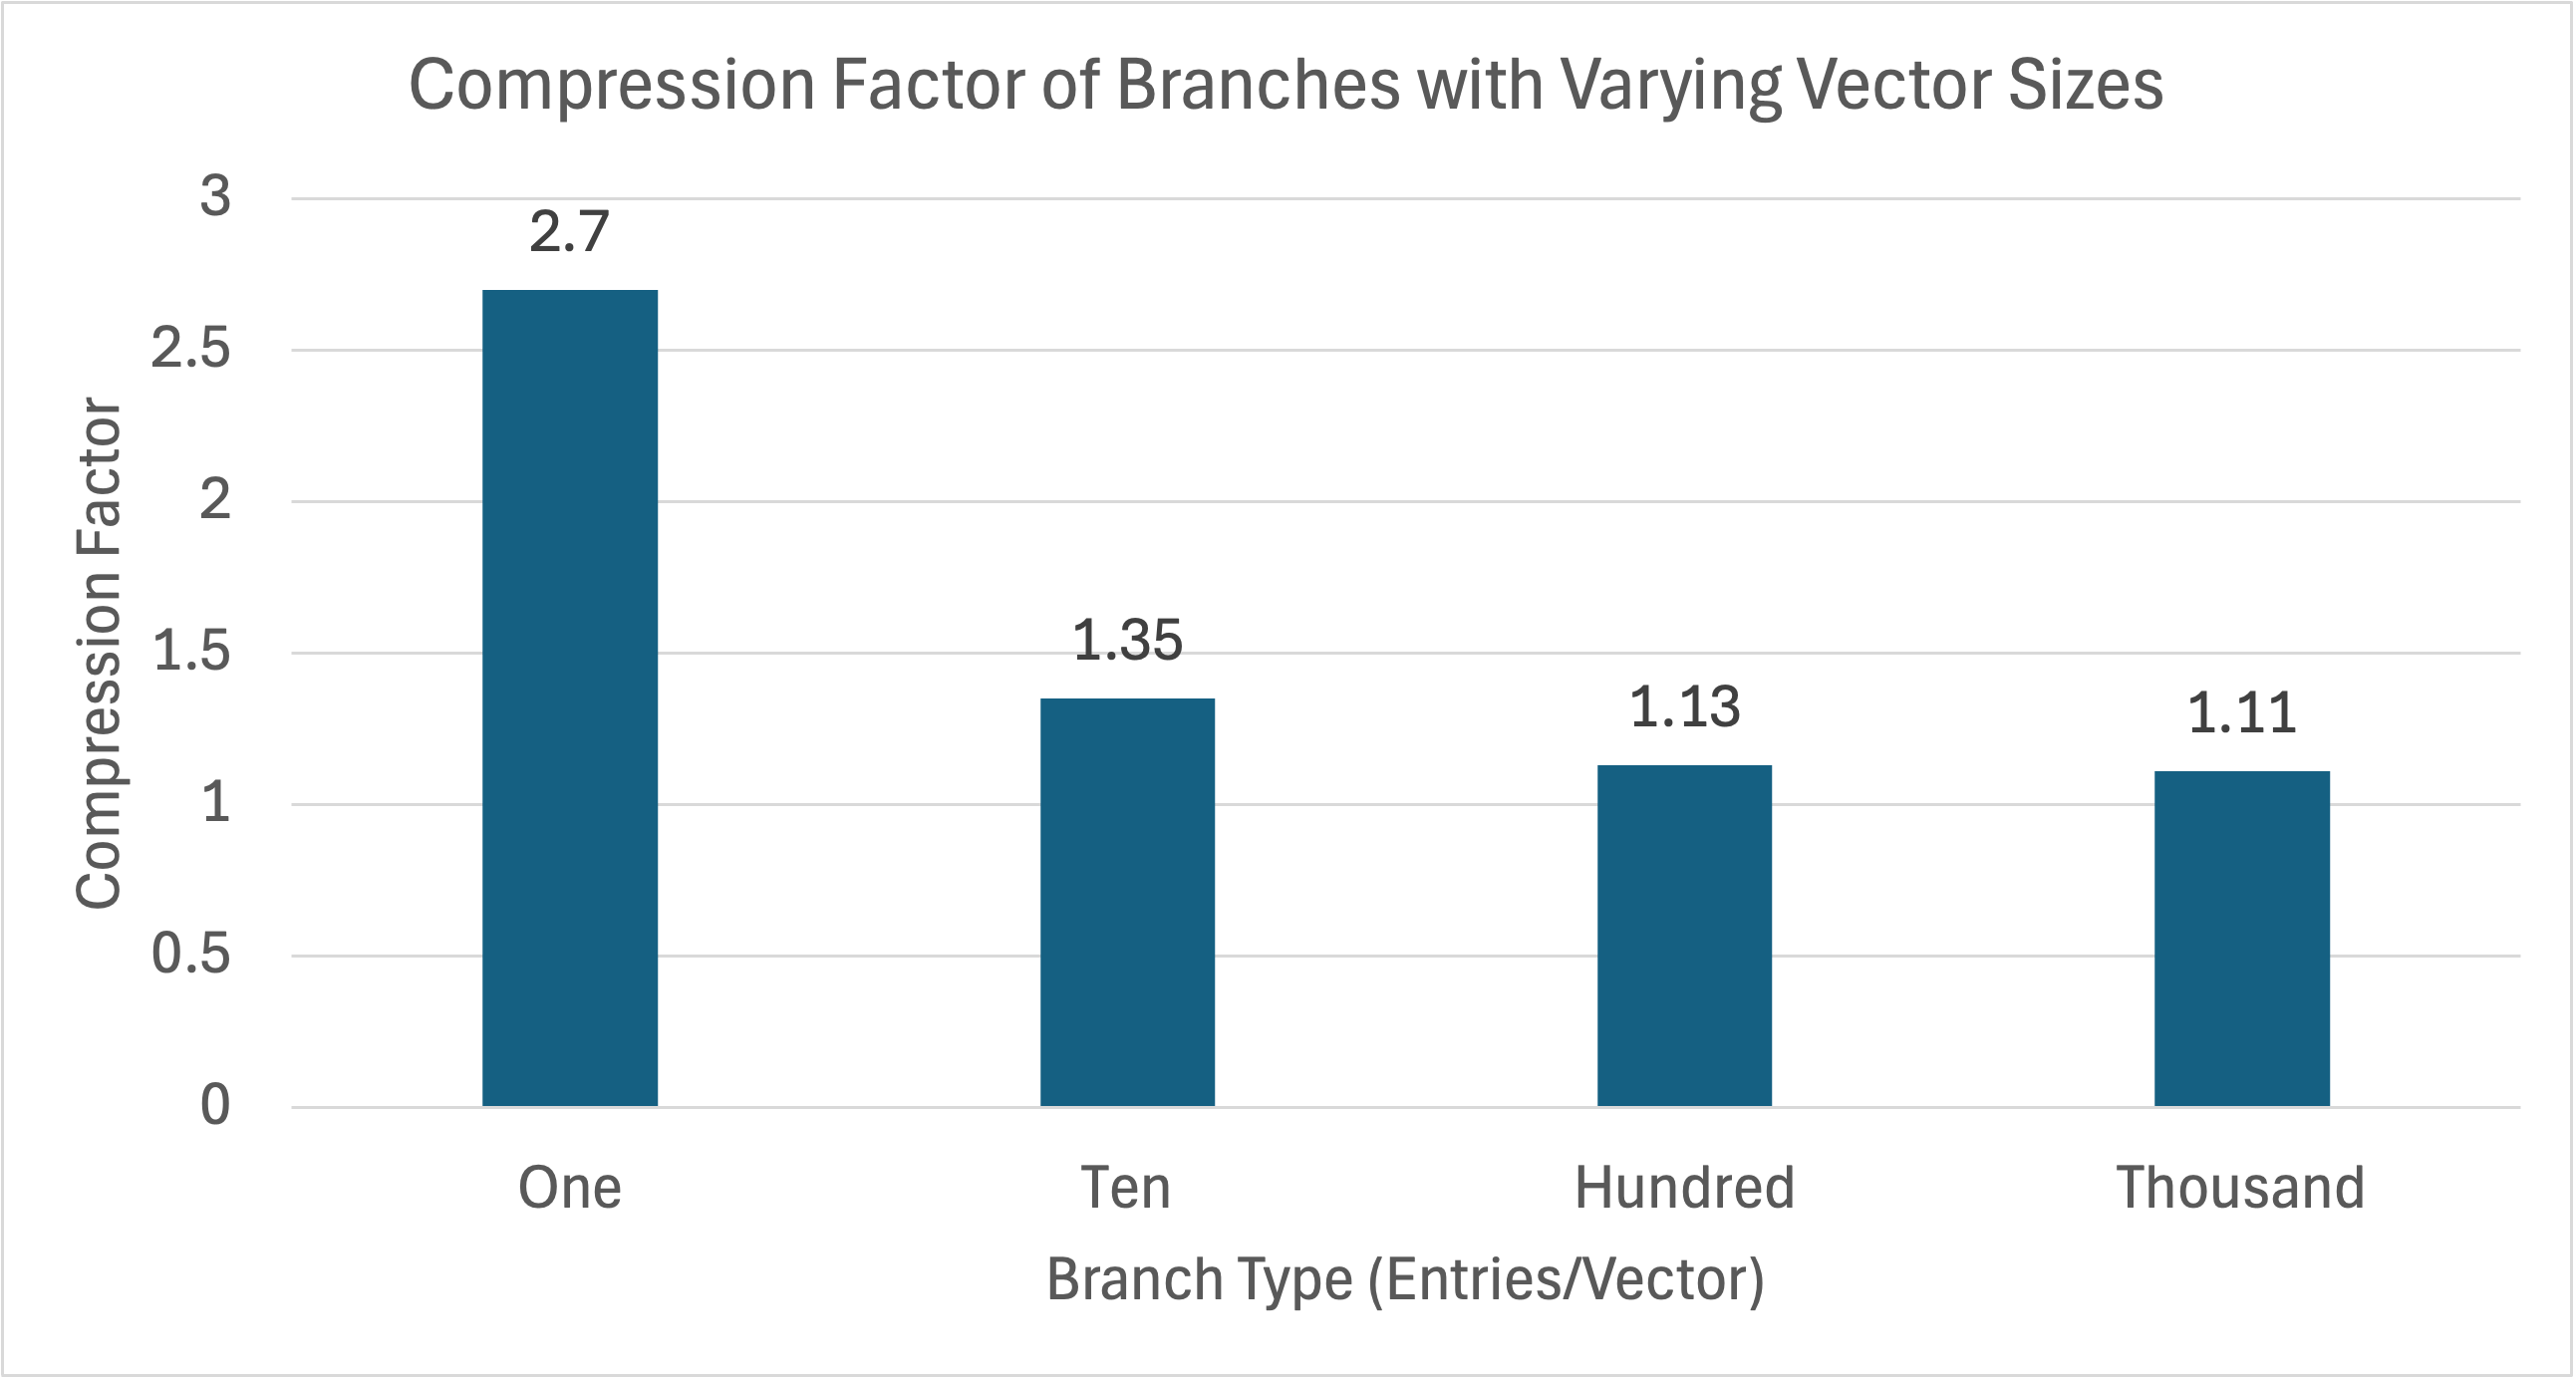
\includegraphics[width=.8\textwidth]{content/toymodel_content/branch_compfacts_nomix.png}
    \caption{Compression factors of $N=1000$ entries per branch with random-valued vectors of varying size.}
    \label{fig:toymodel_compF_rndm_vectors}
\end{figure}

% \begin{figure}[h]
%     \caption{File size of $N=1000$ entries per branch with random-valued vectors of varying size.}
%     \label{fig:toymodel_filesize_rndm_vectors}
%     \centering
%     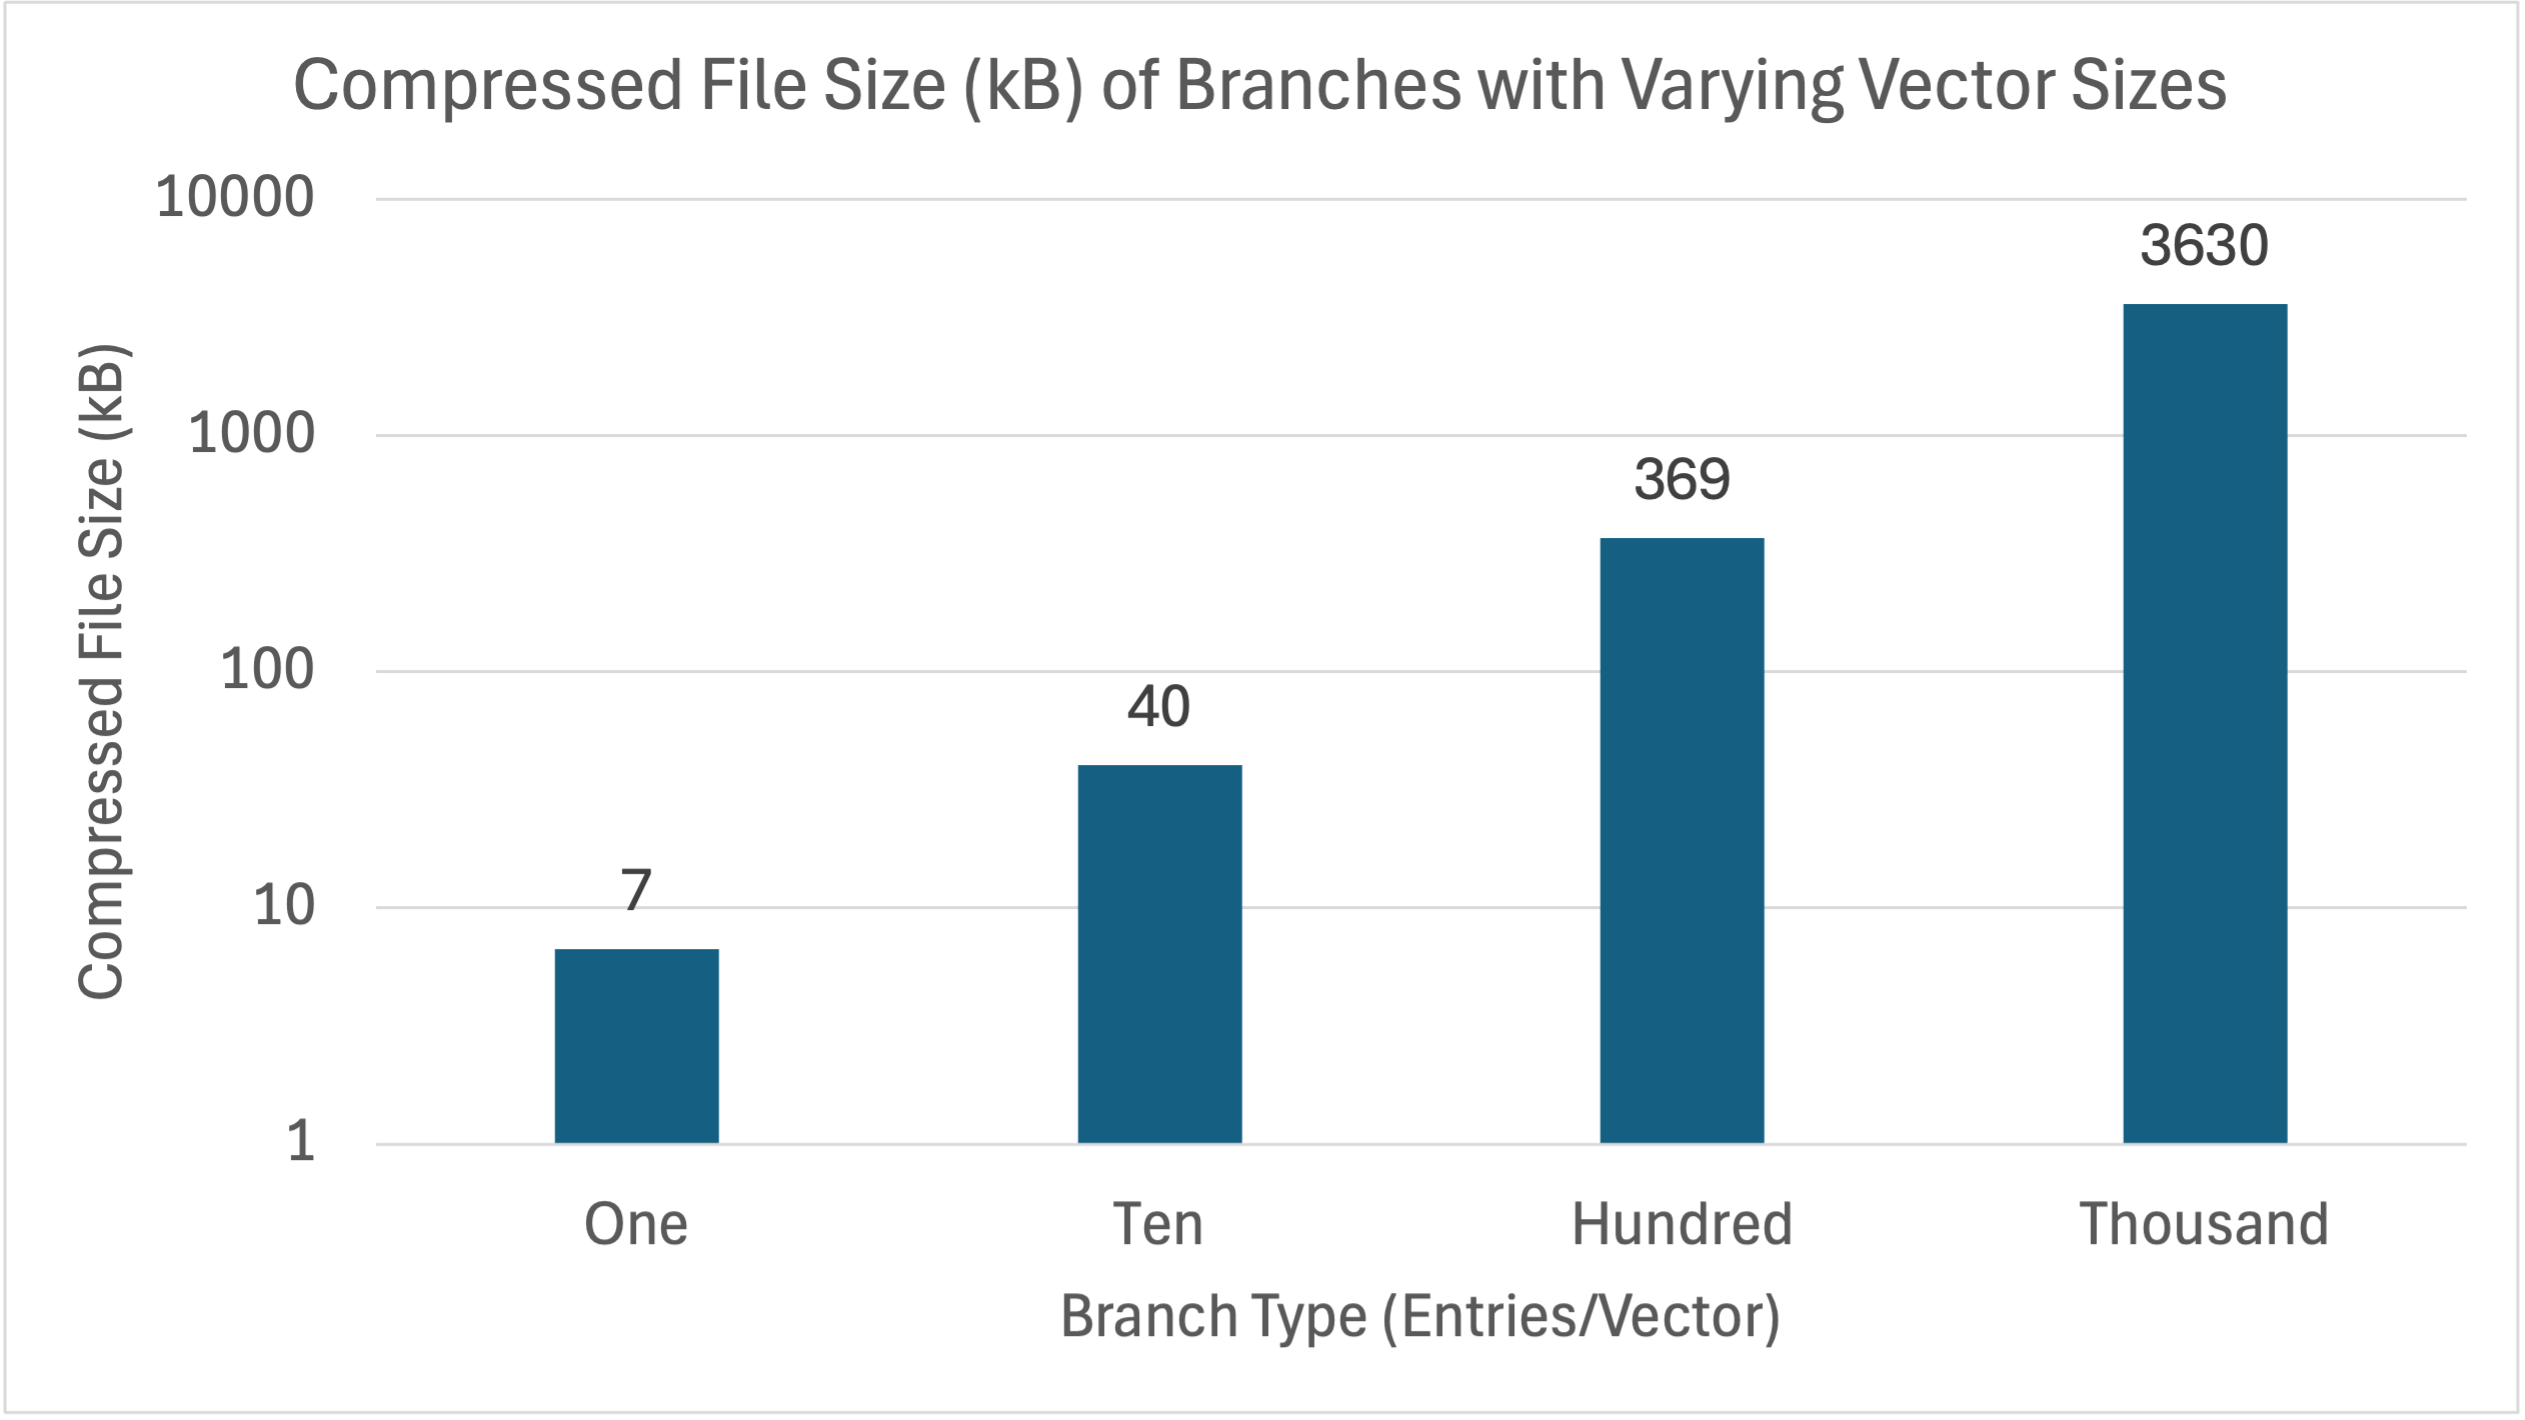
\includegraphics[width=.8\textwidth]{content/toymodel_content/branch_fileSize_nomix.png}
% \end{figure}

Figure \ref{fig:toymodel_compF_rndm_vectors} shows compression drop-off as the branches with more randomized floats per vector were present.
This is the leading indication that there needs to be more compressible data within the branches. 

\subsection{Mixed-Random Float Branches}
The branches needed to have some balance between compressible and incompressible data to mimic the compression ratio found in real data.
How this was achieved was by filling each vector with different ratios of random floats and repeating integers, which will now be described in detail.

The first change was increasing the total number of events per branch from $N = 10^4$ to $N = 10^5$. 
Mixing of random floats and repeated integer values takes the same script structure as Section \ref{sec:toy_compression_random_float_branches} but adjusts the event generation loop.
\begin{lstlisting}[language=C]  
  void VectorTree() {
    ...
    // Events Loop
    for (int j = 0; j < N; j++) {
        // Clearing entries from previous iteration
        vec_ten0.clear();
        vec_ten1.clear();
        vec_ten2.clear();
        vec_ten3.clear();

        // Generating vector elements, filling vectors
        // Generating vec_ten0
        // Contents of the vector:
        //    {float_0}
        //    Only one float of random value
        // And since there's only one entry, we don't mix the entries. 
        float_0 = gRandom->Gaus(0, 1) * gRandom->Rndm();
        vec_ten0.emplace_back(float_0);
        

        // Generating vec_ten1
        // Contents of the vector:
        //    {float_1_0, float_1_1, float_1_2, float_1_3, float_1_4, 1, 1, 1, 1, 1}
        //    5 floats of random values, 5 integers of value 1.
        for (int b = 0; b < size_vec_1; b++) {
            if (b < size_vec_1 / 2) {
              float_1 = gRandom->Rndm() * gRandom->Gaus(0, 1);
              vec_ten1.emplace_back(float_1);
            } else {
              float_1 = 1;
              vec_ten1.emplace_back(float_1);
            }
        }

        // Do the same with vec_ten2 and vec_ten3, except for 
        //     vectors with size 100 and 1000 respectively. 


        // After all branches are filled, fill the TTree with 
        //     new branches
        tree->Fill(); 
    }
    // Saving tree and file
    tree->Write();
    ...
  }
\end{lstlisting}

As shown in the \verb|if|-statements in line \verb|25|, if the iterator was less than half of the total number of entries in the vector then that entry had a randomized float put in that spot in the vector, otherwise it would be filled with the integer \verb|1|.
Having a mixture of half random floats and half integer \verb|1| led to the larger branches still seeing poor compression, so a new mixture of 1/4 random data was introduced. 
Even though $N=10^5$ had the larger branches closer to the desired compression ratio, testing at $N=10^6$ events improves the accuracy of the overall file size to more closely resemble real data.

Figure \ref{fig:toymodel_compF_1e6_mix_random} shows the difference between compression between the two mixtures at $N=10^6$ events. 
When the number of events is increased from $N=10^5$ to $N=10^6$, at the 1/2 random-mixture, the branches with more than one entry per vector see their compression factor worsen. 
Figure \ref{fig:toymodel_compF_1e5_mix_random} shows a compression ratio hovering around 3 for the larger branches, whereas Figure \ref{fig:toymodel_compF_1e6_mix_random} shows the same branches hovering around 2. 

\begin{figure}[h]
    \centering
    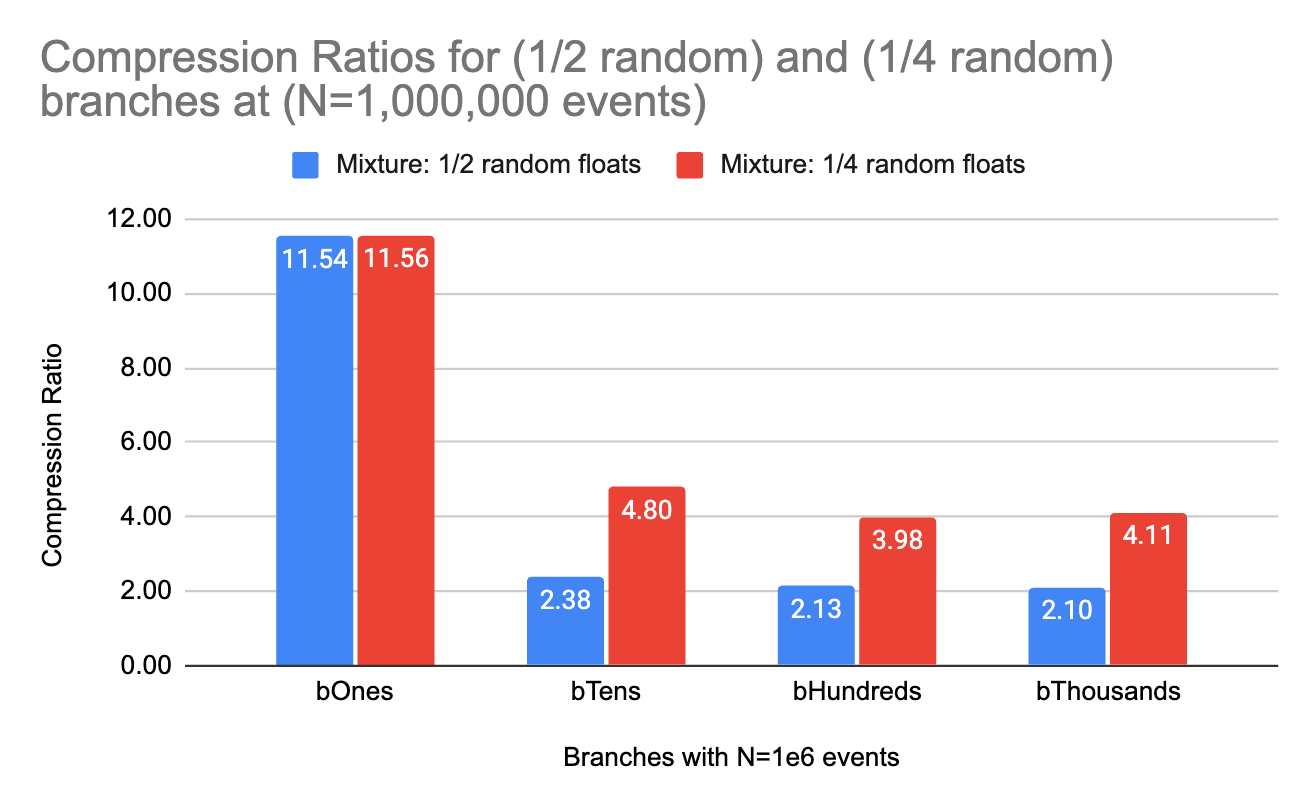
\includegraphics[width=.8\textwidth]{content/toymodel_content/Compression Ratios for (1_2 random) and (1_4 random) branches at (N=1,000,000 events).png}
    \caption{Compression Ratios for ($\frac{1}{2}$ random) and ($\frac{1}{4}$ random) branches at ($N=10^6$ events)}
    \label{fig:toymodel_compF_1e6_mix_random}
\end{figure}

\begin{figure}[h]
    \centering
    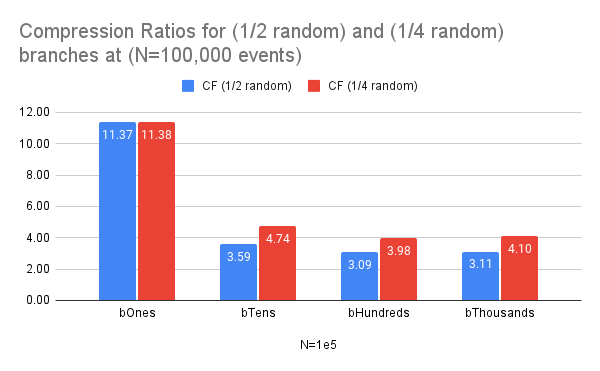
\includegraphics[width=.8\textwidth]{content/toymodel_content/Compression Ratios for (1_2 random) and (1_4 random) branches at (N=100,000 events).png}
    \caption{Compression Ratios for ($\frac{1}{2}$ random) and ($\frac{1}{4}$ random) branches at ($N=10^5$ events)}
    \label{fig:toymodel_compF_1e5_mix_random}
\end{figure}

Unlike the mixture of branches having 1/2 random data, the 1/4 mixture does not see the same compression effect, but with this mixture we see a compression ratio that is in-line with real data.
This is inline with expectation, more repeated integers within the mixture makes the branch more compressible, and the more random floats in the mixture will make the branch more difficult to compress.
With these mixtures added to the toy model, we can start looking at varying the basket sizes to see how they affect compression.

\section{Basket-Size Investigation}
\label{sec: toy-model basket-size investigation}

Investigating how compression is affected by the basket size requires us to change the basket size, refill the branch and read it out.
Changing the basket buffer size was done at the script level with a simple setting after the branch initialization and before the event loop the following code:
\begin{lstlisting}
    int basketSize = 8192000; // 8 MB
    tree->SetBasketSize("*",basketSize);
\end{lstlisting}
This ROOT-level setting was sufficient for the case of the toy model; testing of the basket size setting both at the ROOT- and Athena-level would be done later using derivation production jobs in Section \ref{sec:DAODProd_Analysis}.
The lower bound set for the basket size was 1 kB and the upper bound was 16 MB.
The first branch looked at closely was the branch with a thousand vectors with half of them being random floats, see Figure \ref{fig:toymodel_CFvsBranchSize_1/2mixture}.

\begin{figure}[h]
    \centering
    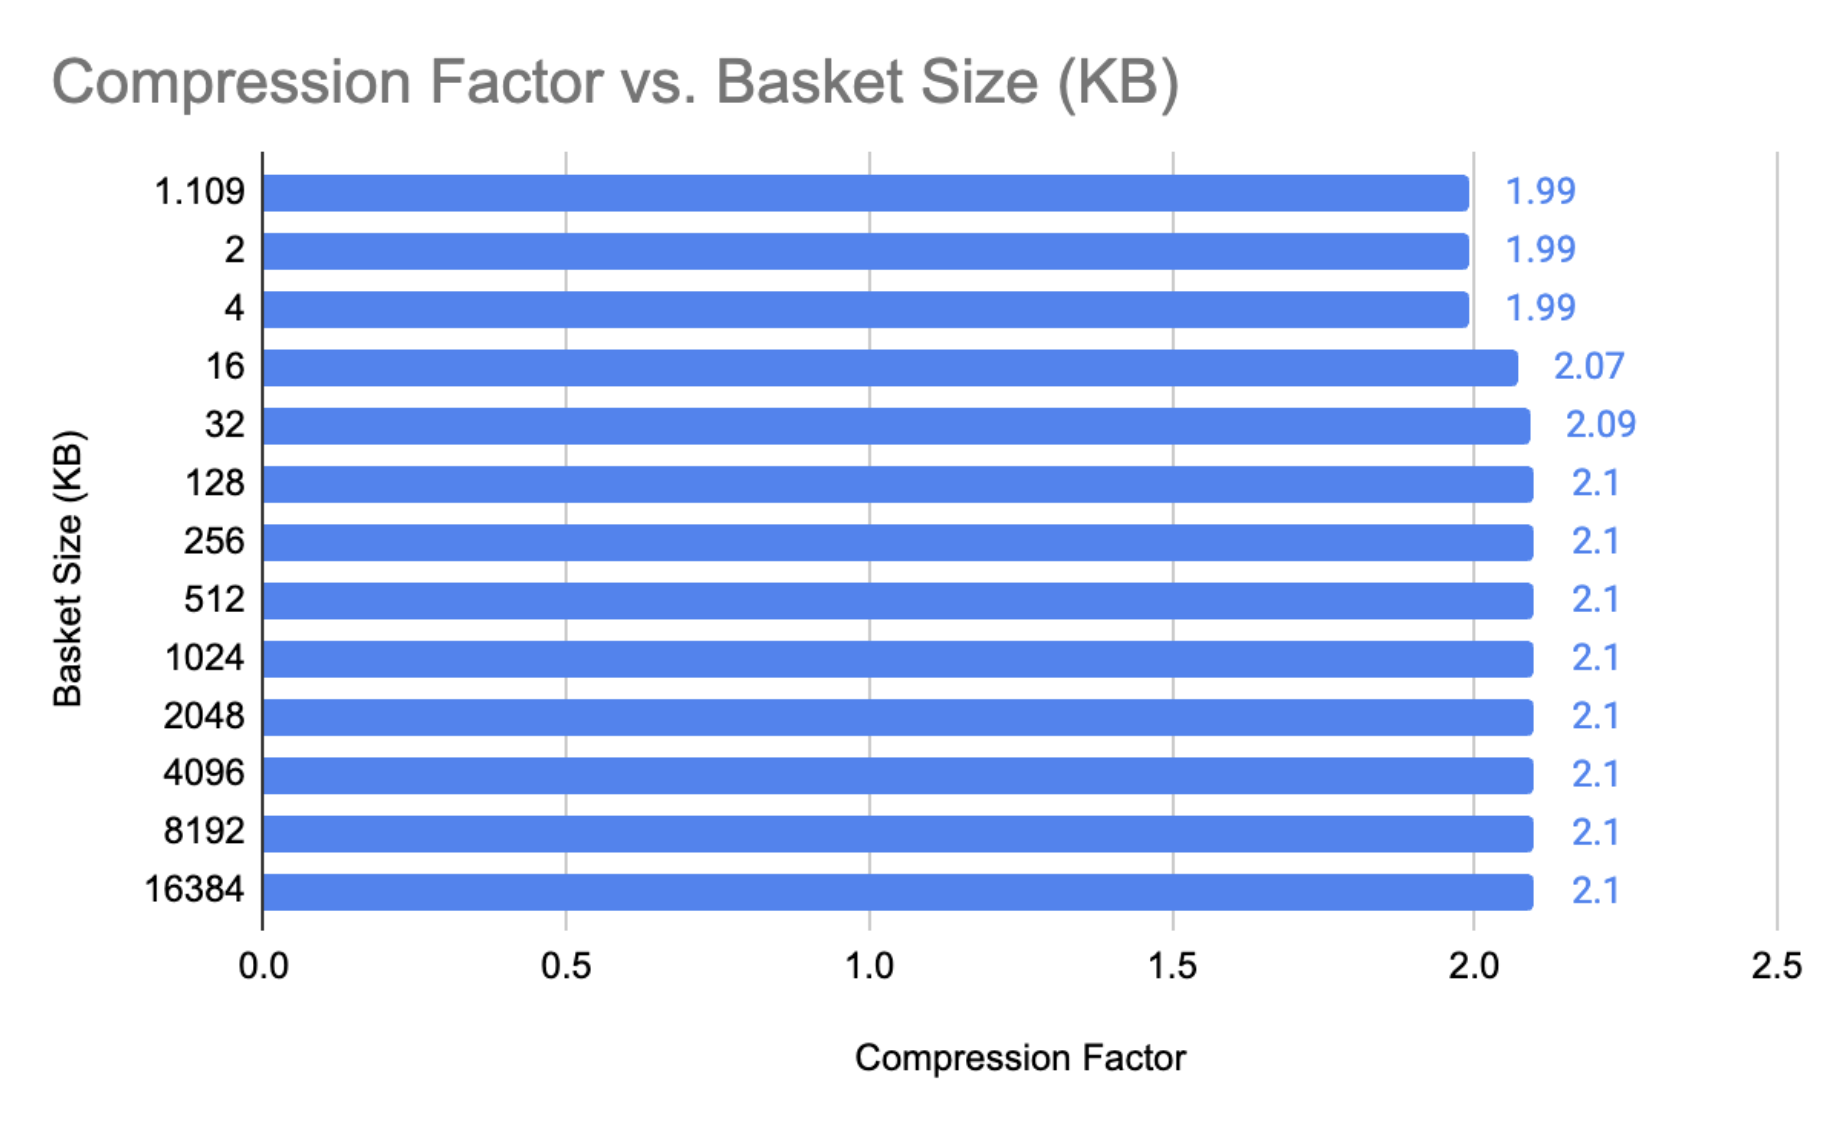
\includegraphics[width=.8\textwidth]{content/toymodel_content/Compression Factor vs. Branch Size (KB).png}
    \caption{Compression Factors vs Branch Size (1000 entries per vector, 1/2 Mixture $N=10^6$ events)}
    \label{fig:toymodel_CFvsBranchSize_1/2mixture}
\end{figure}

\begin{figure}[h]
    \centering
    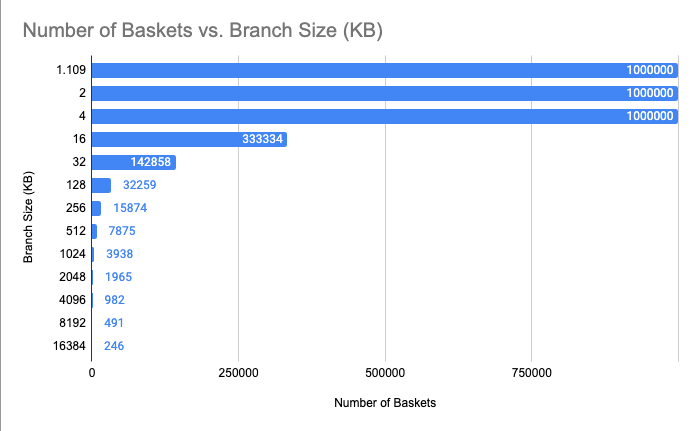
\includegraphics[width=.8\textwidth]{content/toymodel_content/Number of Baskets vs Branch Size.png}
    \caption{Number of Baskets vs Branch Size (1000 entries per vector, 1/2 Mixture $N=10^6$ events)}
    \label{fig:toymodel_NumBasketsvsBranchSize_1/2mixture}
\end{figure}

Figures \ref{fig:toymodel_CFvsBranchSize_1/2mixture} and \ref{fig:toymodel_NumBasketsvsBranchSize_1/2mixture} are the first indication that the lower basket sizes are too small to effectively compress the data. 
For baskets smaller than 16 kB, it is necessary to have as many baskets as events to store all the data effectively.
For a mixed-content vector with one thousand entries, containing 500 floats and 500 integers (both are 4 bytes each), its size is approximately 4 kB.
ROOT creates baskets of at least the size of the smallest branch entry, in this case the size of a single vector.
So even though the basket size was set to 1 or 2 kB, ROOT created baskets of 4 kB.
These baskets less than or equal to $4$kB have a significantly worse compression than the baskets greater than $4$kB in size, so the focus was shifted toward baskets.  
Once the basket size is larger than the size of a single vector, more than one vector can be stored in a single basket and the total number of baskets is reduced.

There were different types of configuration to the toy model investigated by this study. 
Looking further into the types of mixtures and how they would affect compression are shown in Figures \ref{fig:toymodel_328_compF_vs_basketsize} and \ref{fig:toymodel_418_compF_vs_basketsize}. 
Here the same mixtures were used but the precision of the floating point numbers was decreased from the standard 32 floating-point precision to 16 and 8, making compression easier. 

\begin{figure}[h]
    \centering
    \begin{subfigure}{.5\textwidth}
        \centering
        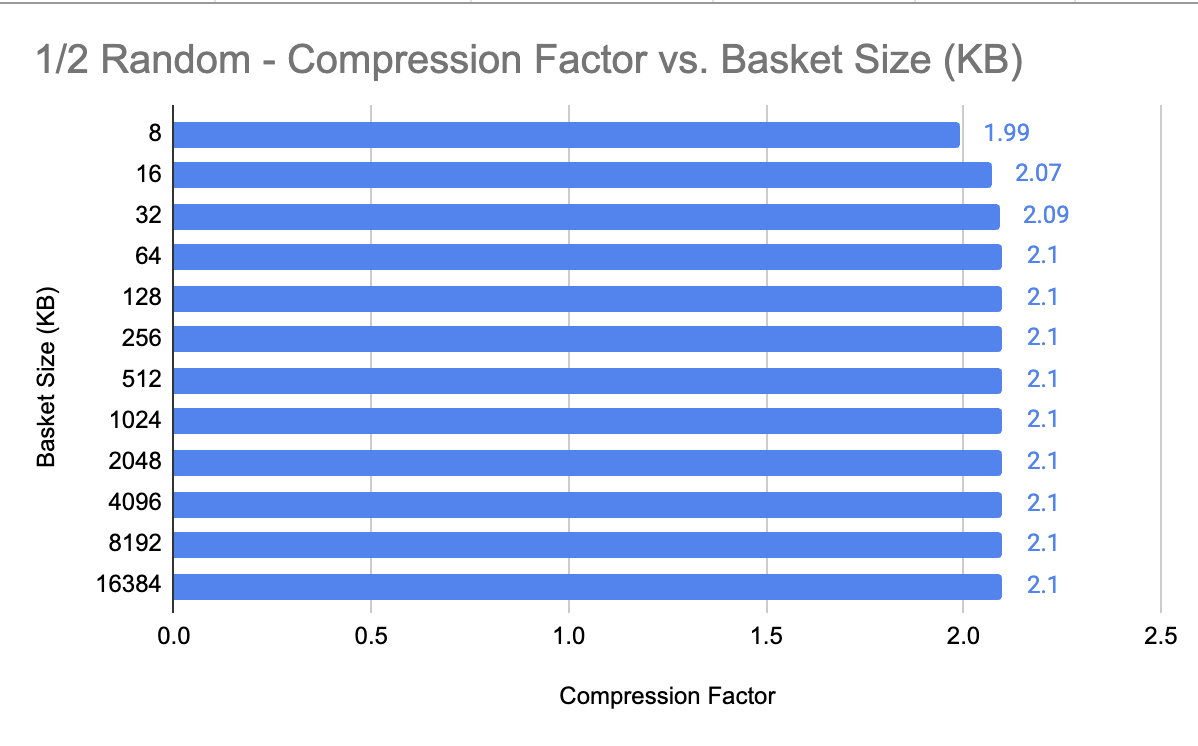
\includegraphics[width=\textwidth]{content/toymodel_content/3.28/1_of_2.png}
        % \caption{A subfigure}
        \label{fig:toymodel_328_compF_vs_basketsize_subA}
      \end{subfigure}%     
      \begin{subfigure}{.5\textwidth}
        \centering
        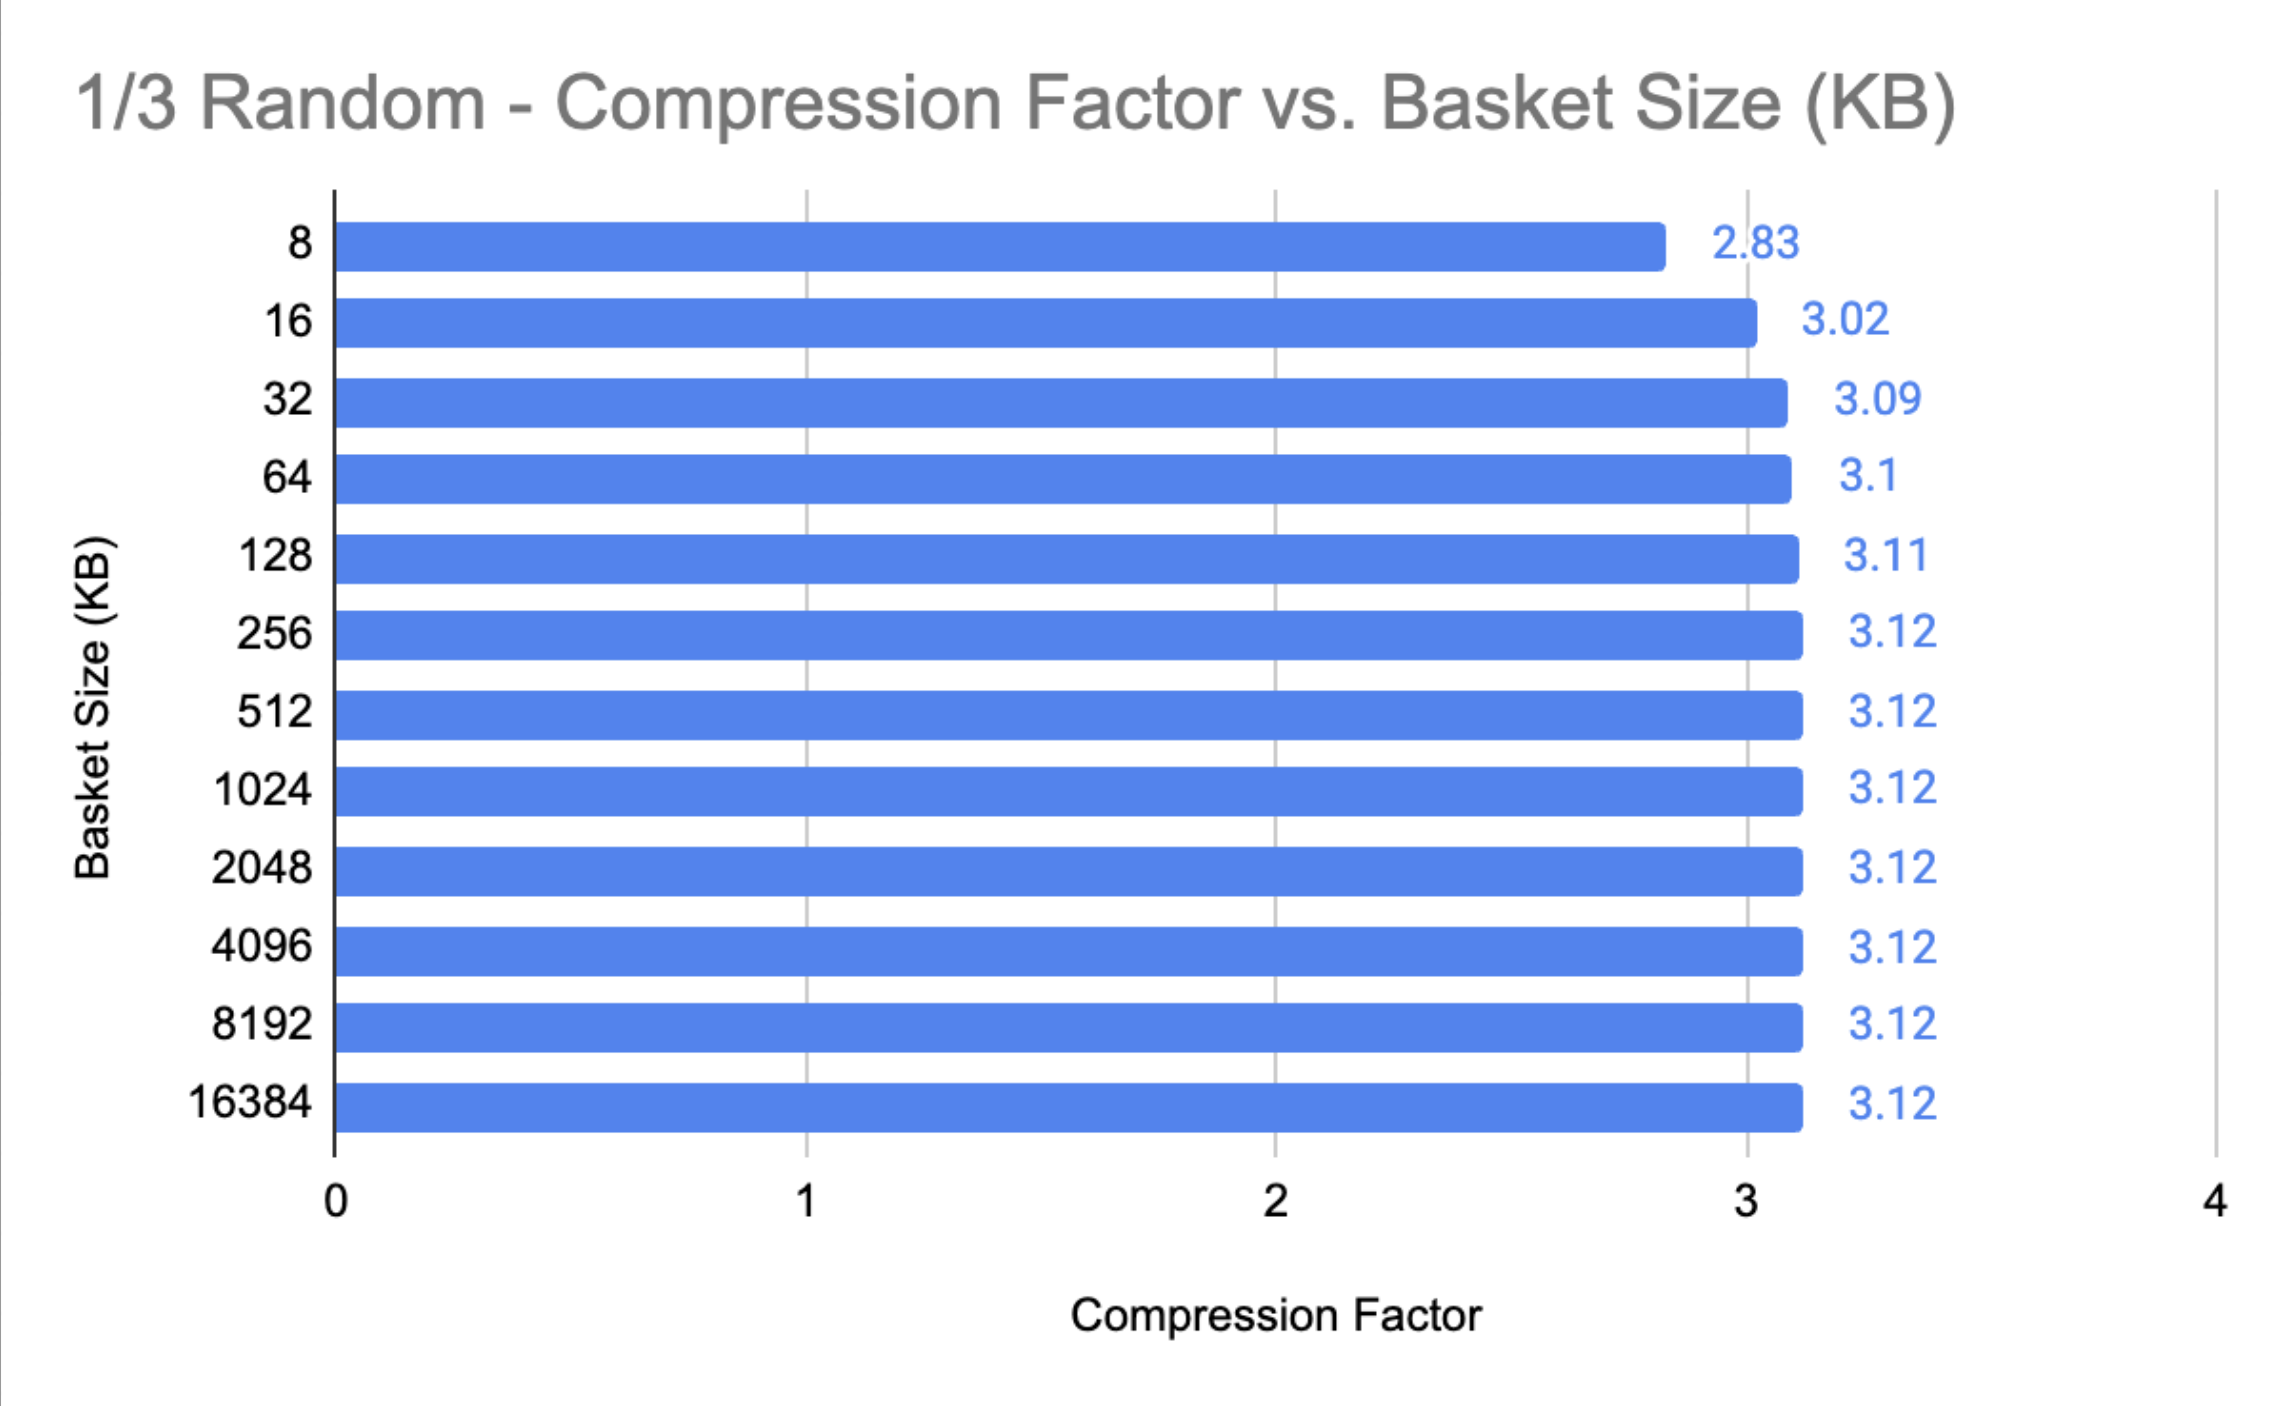
\includegraphics[width=\textwidth]{content/toymodel_content/3.28/1_of_3.png}
        % \caption{B subfigure}
        \label{fig:toymodel_328_compF_vs_basketsize_subB}
      \end{subfigure}% 
      \linebreak
      \begin{subfigure}{.5\textwidth}
        \centering
        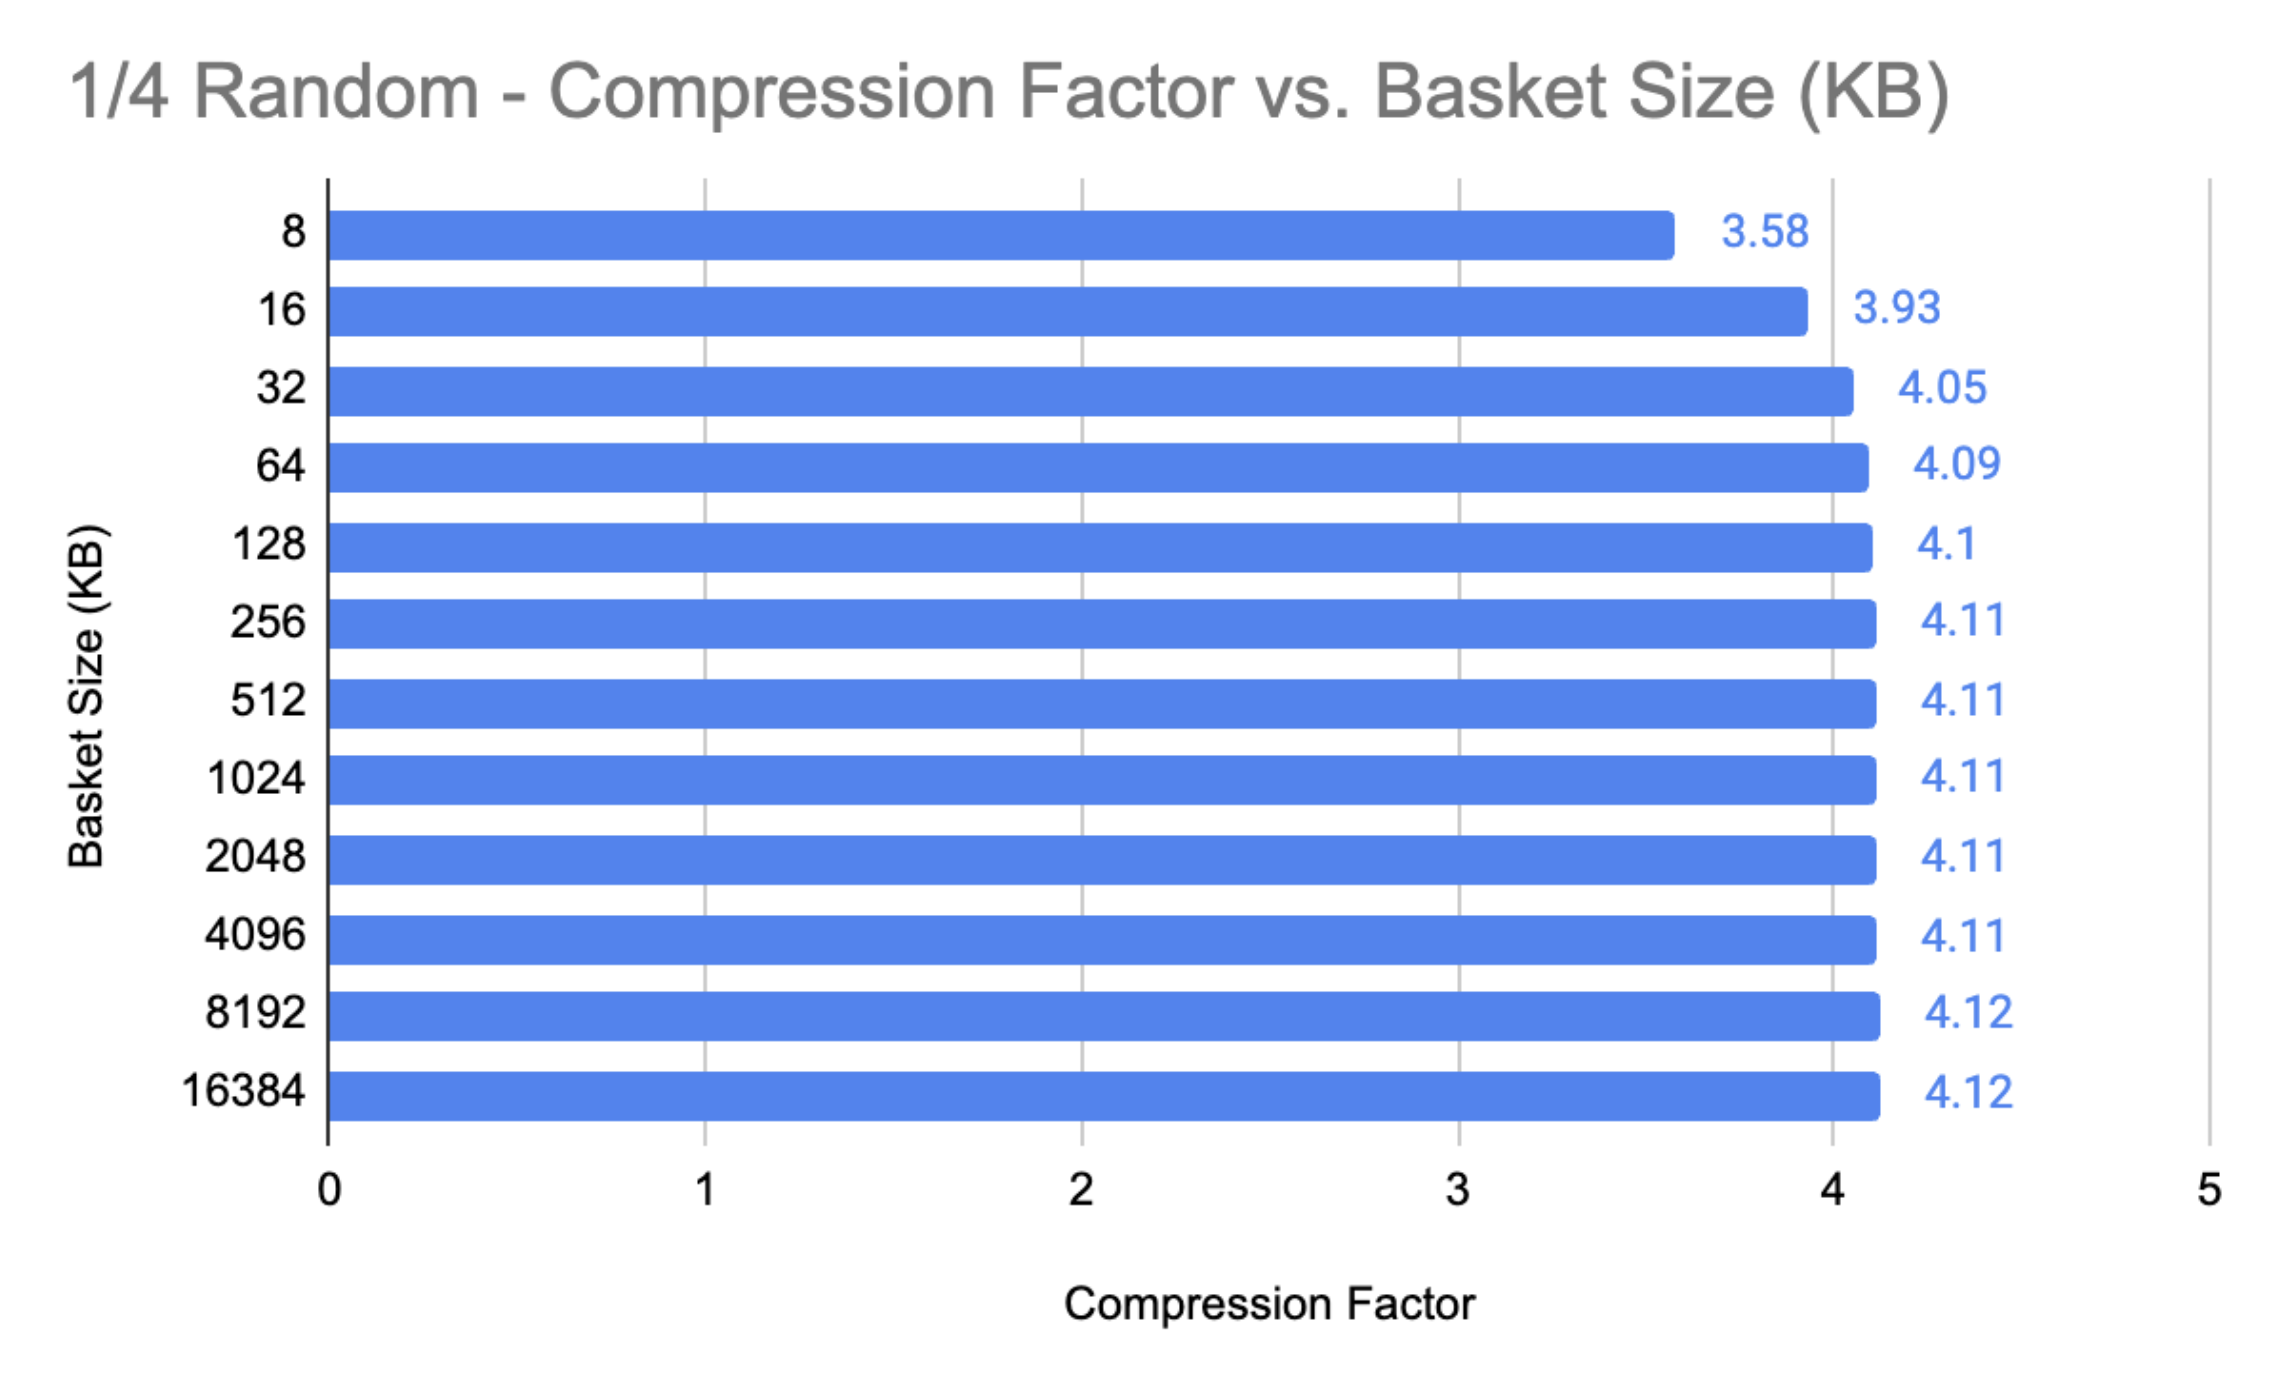
\includegraphics[width=\textwidth]{content/toymodel_content/3.28/1_of_4.png}
        % \caption{C subfigure}
        \label{fig:toymodel_328_compF_vs_basketsize_subC}
      \end{subfigure}% 
      \begin{subfigure}{.5\textwidth}
        \centering
        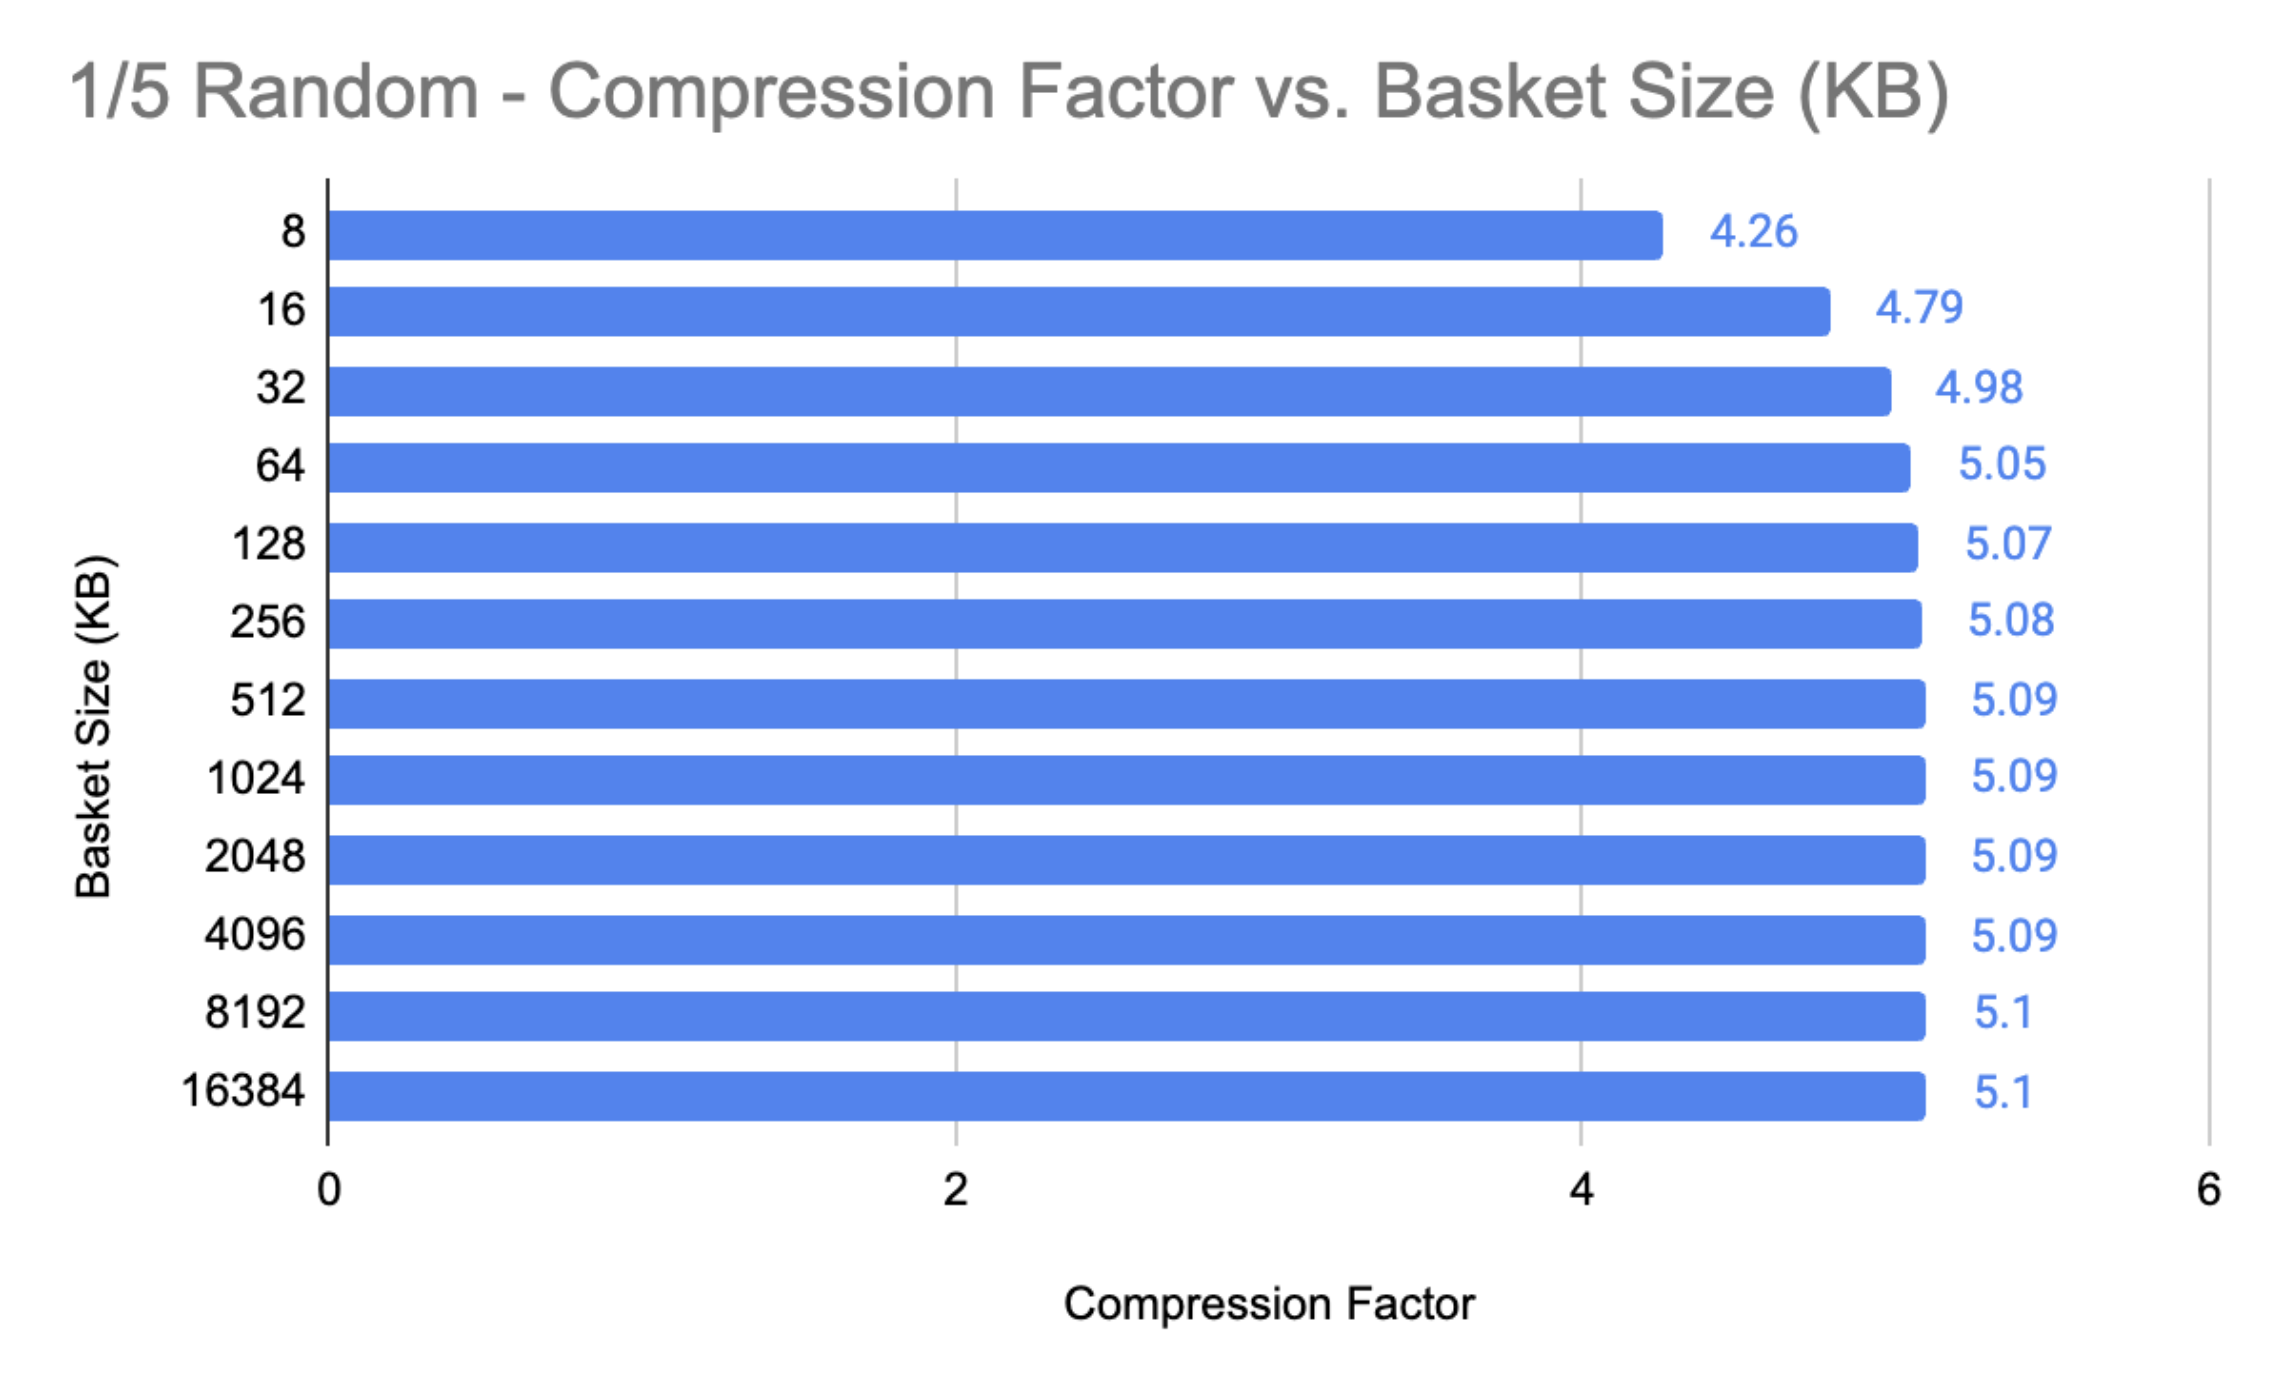
\includegraphics[width=\textwidth]{content/toymodel_content/3.28/1_of_5.png}
        % \caption{D subfigure}
        \label{fig:toymodel_328_compF_vs_basketsize_subD}
      \end{subfigure}% 
    \caption{Varying Mixtures in 8 point precision - Number of Baskets vs Branch Size ($N=10^6$ events)}
    \label{fig:toymodel_328_compF_vs_basketsize}
\end{figure}

\begin{figure}[h]
    \centering
    \begin{subfigure}{.5\textwidth}
        \centering
        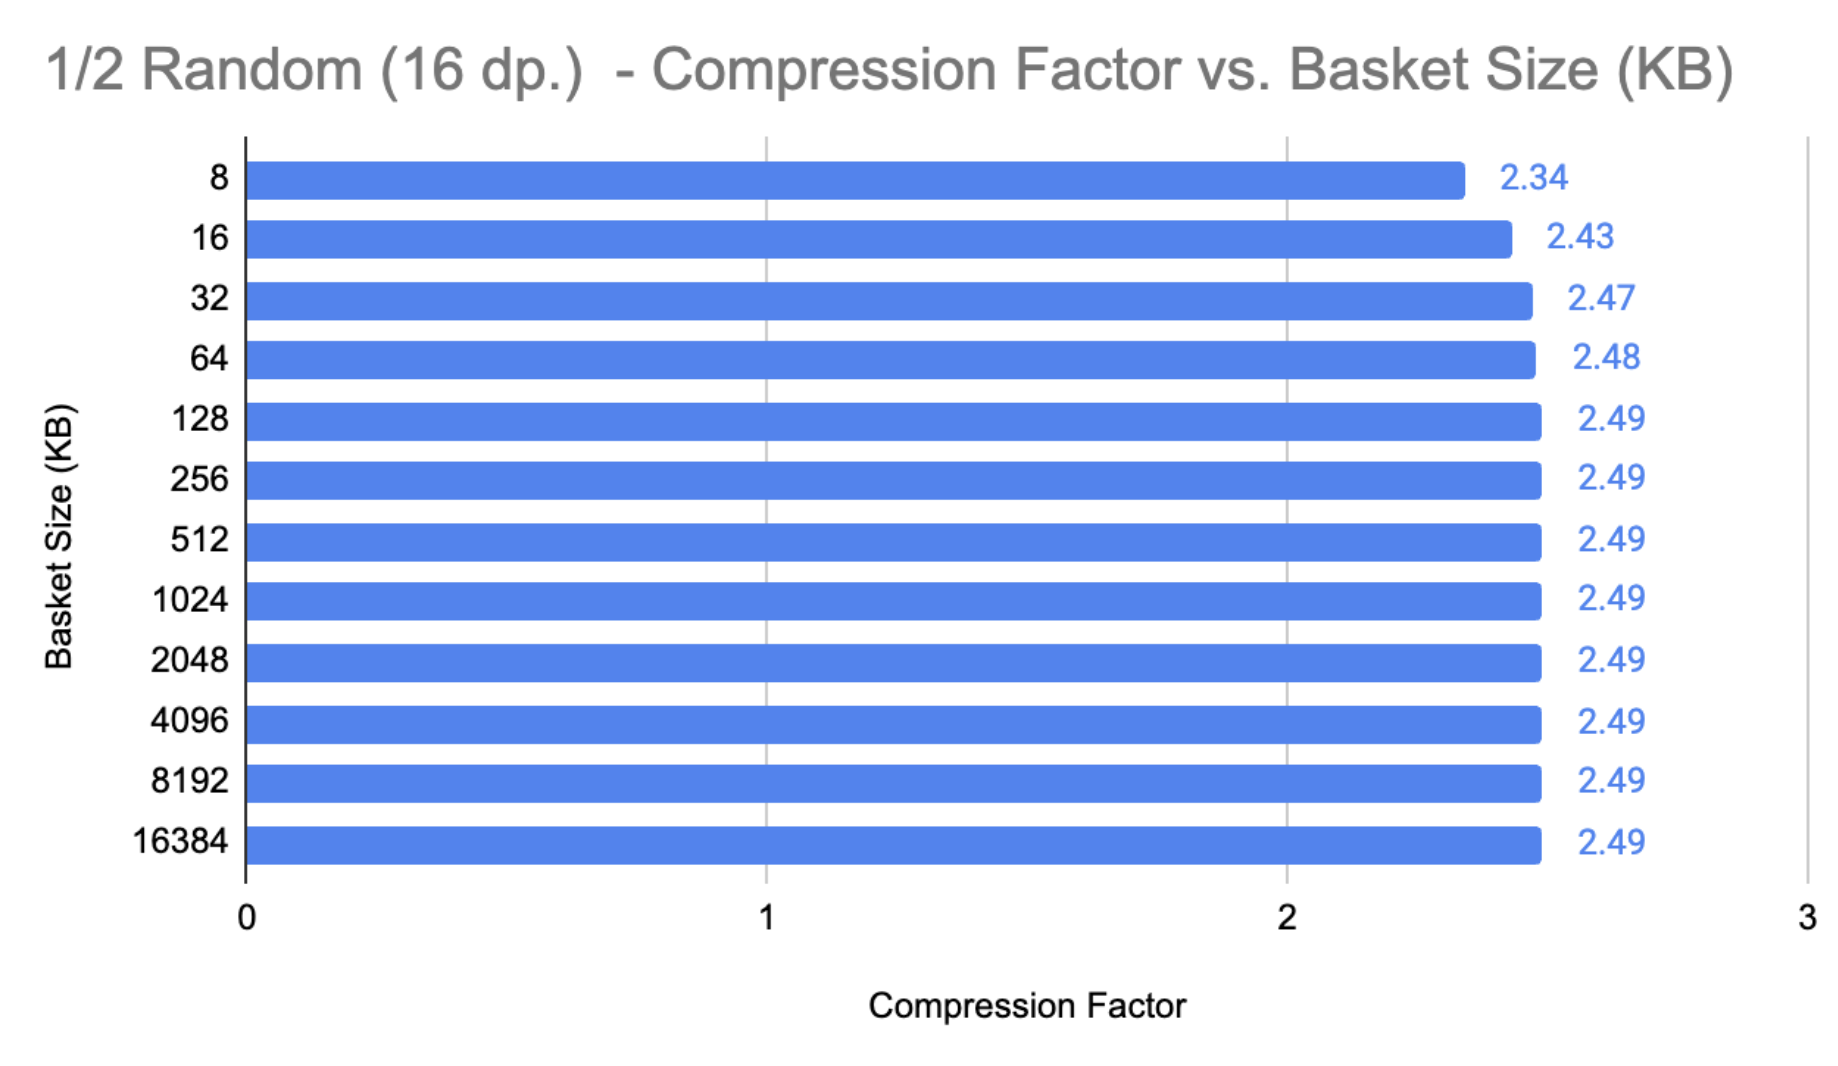
\includegraphics[width=\textwidth]{content/toymodel_content/4.18/1_of_2.png}
        % \caption{A subfigure}
        \label{fig:toymodel_418_compF_vs_basketsize_subA}
      \end{subfigure}%     
      \begin{subfigure}{.5\textwidth}
        \centering
        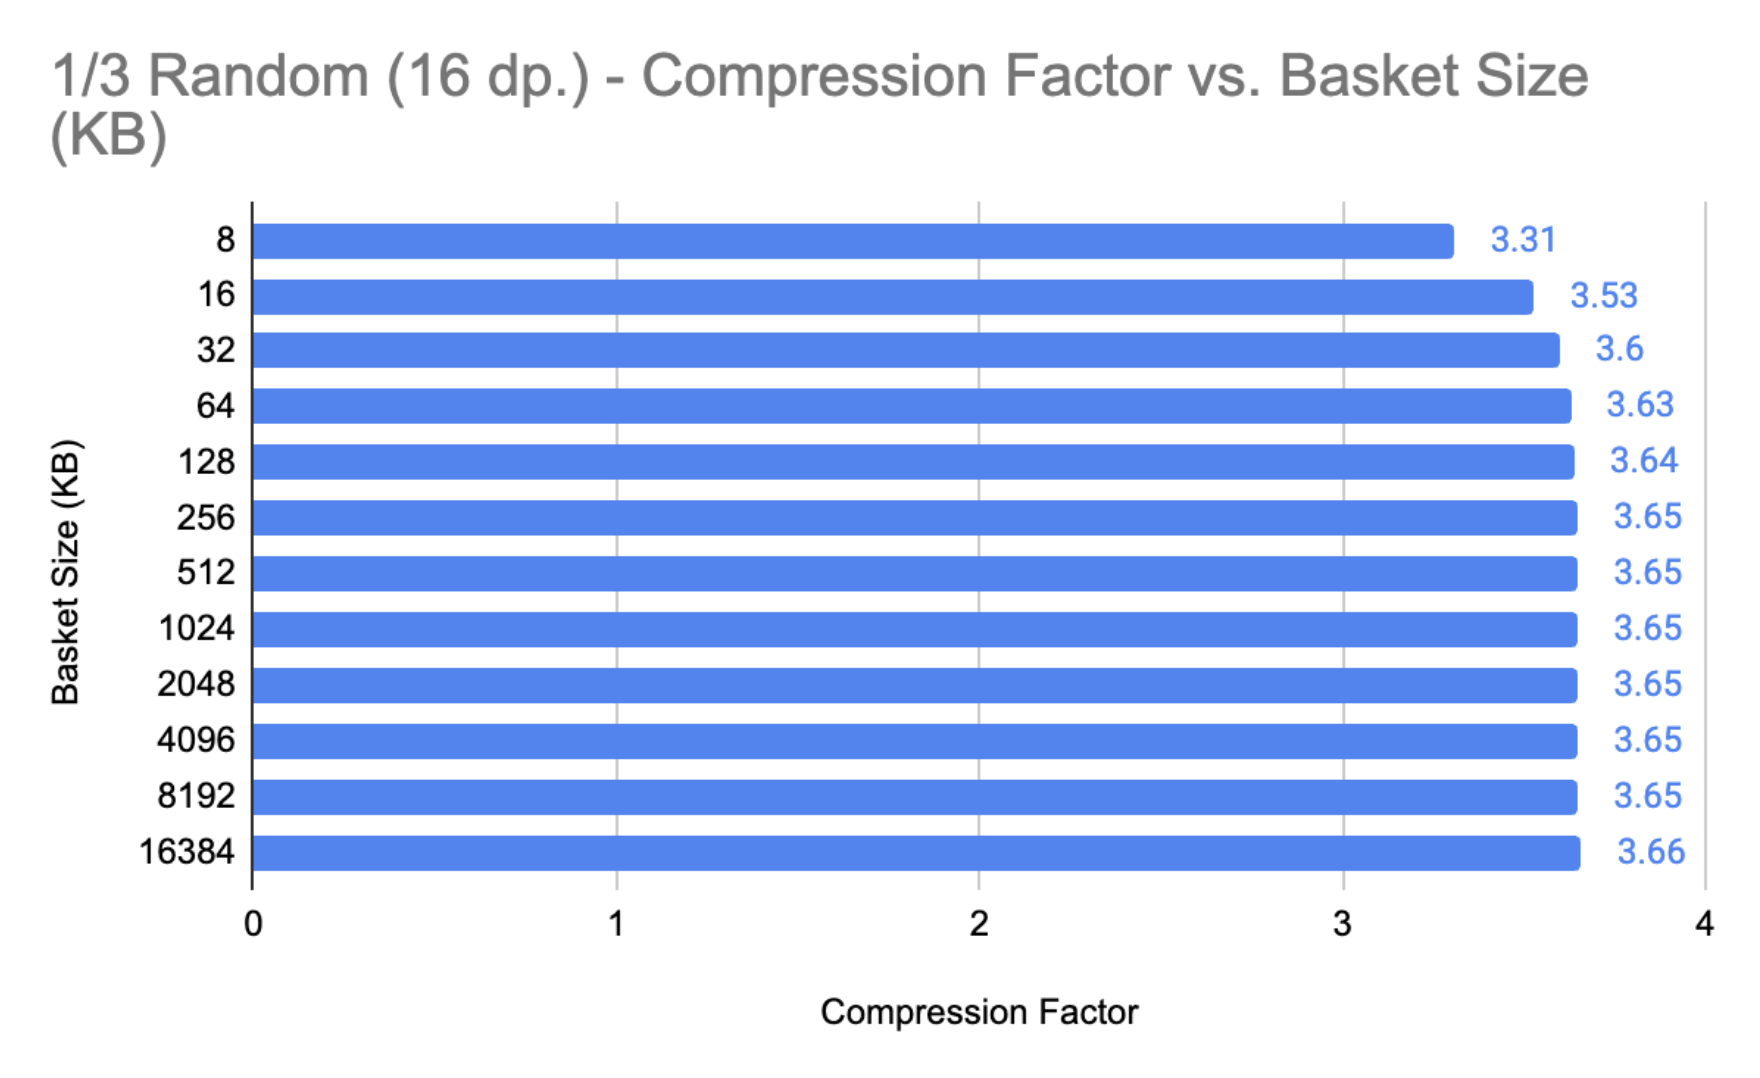
\includegraphics[width=\textwidth]{content/toymodel_content/4.18/1_of_3.png}
        % \caption{B subfigure}
        \label{fig:toymodel_418_compF_vs_basketsize_subB}
      \end{subfigure}% 
      \linebreak
      \begin{subfigure}{.5\textwidth}
        \centering
        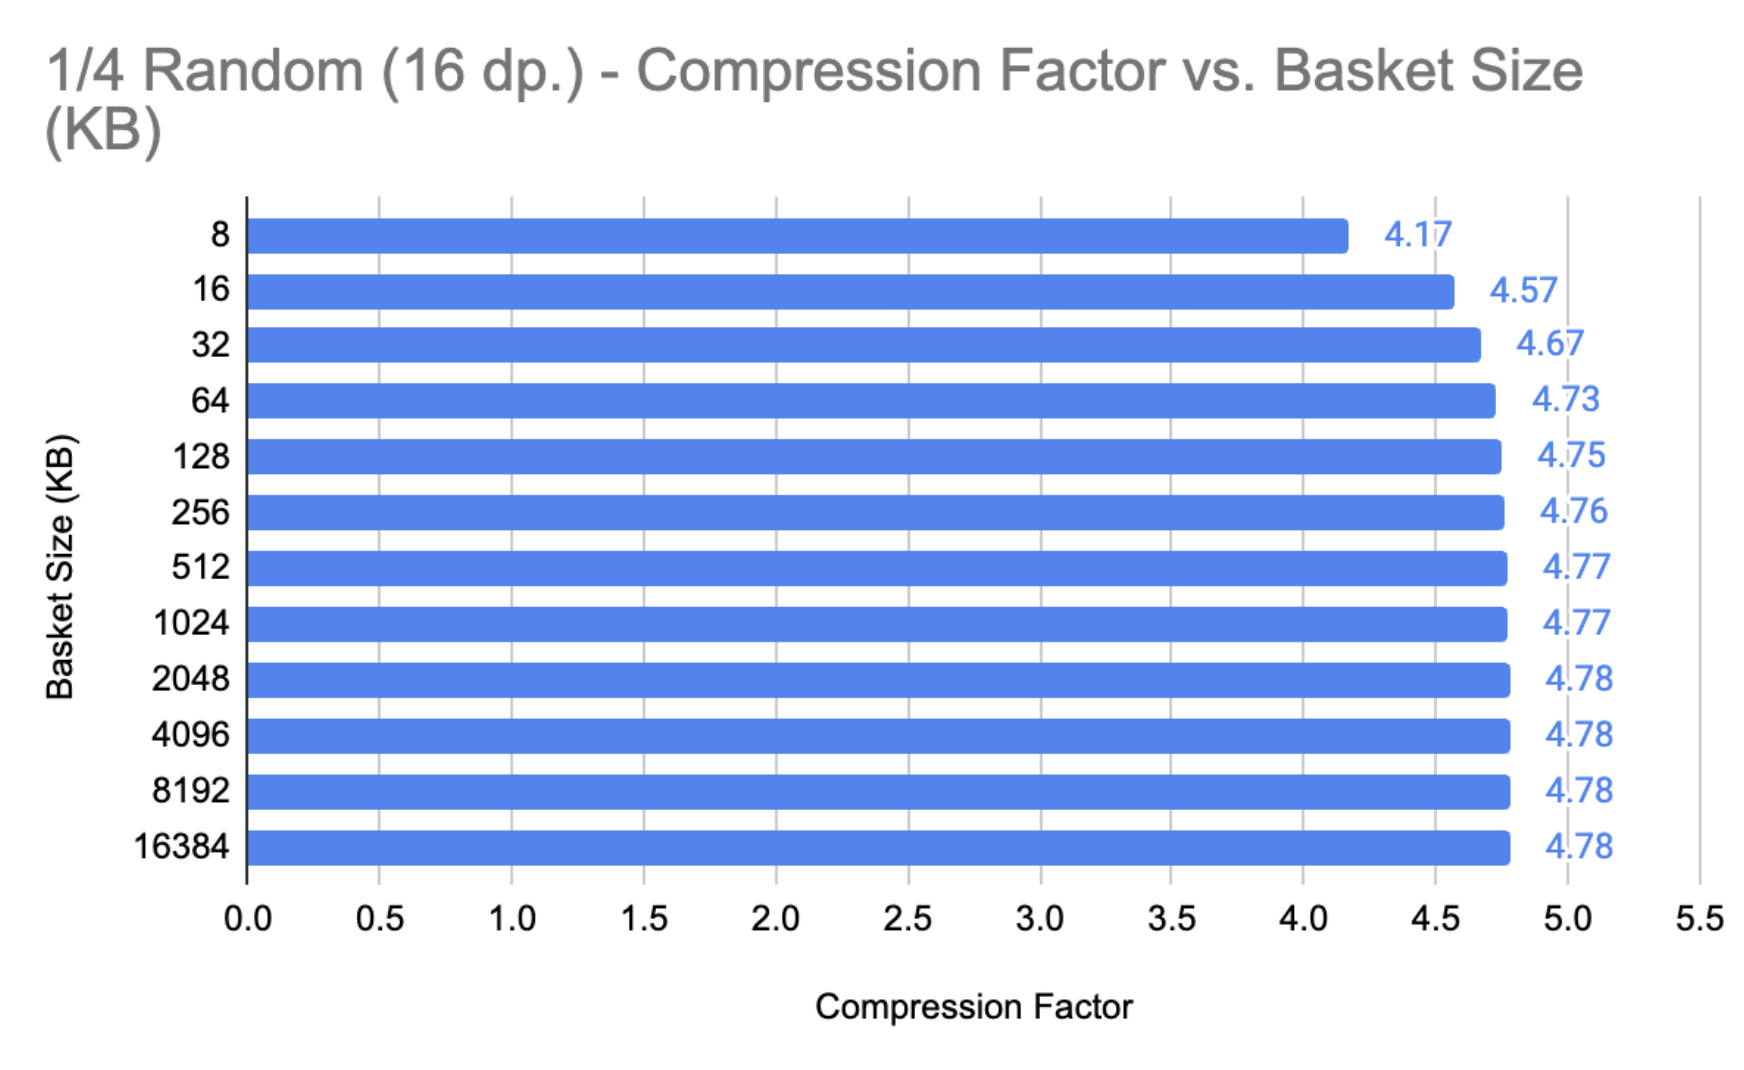
\includegraphics[width=\textwidth]{content/toymodel_content/4.18/1_of_4.png}
        % \caption{C subfigure}
        \label{fig:toymodel_418_compF_vs_basketsize_subC}
      \end{subfigure}% 
      \begin{subfigure}{.5\textwidth}
        \centering
        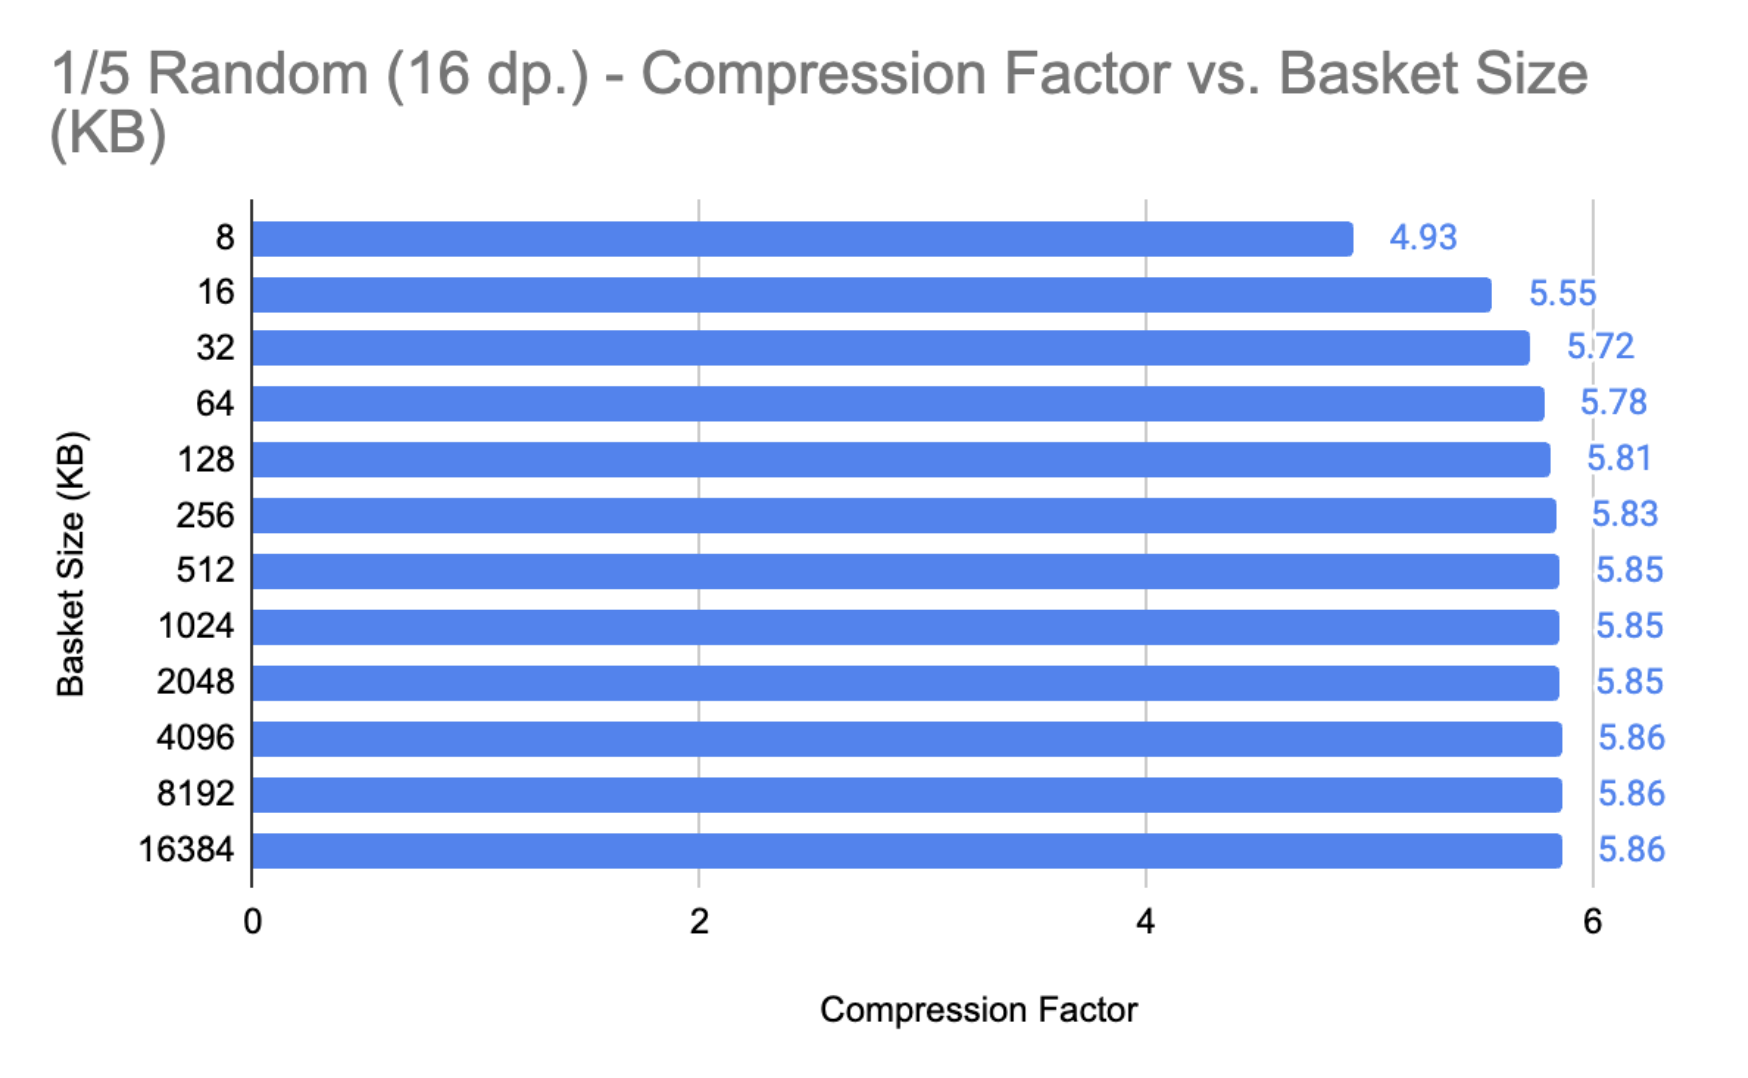
\includegraphics[width=\textwidth]{content/toymodel_content/4.18/1_of_5.png}
        % \caption{D subfigure}
        \label{fig:toymodel_418_compF_vs_basketsize_subD}
      \end{subfigure}% 
      \caption{Varying Mixtures in 16 point precision - Number of Baskets vs Branch Size ($N=10^6$ events)}
      \label{fig:toymodel_418_compF_vs_basketsize}
\end{figure}


Each of these sets of tests indicate that after a certain basket size, i.e. 128 kB, there is no significant increase in compression. 
Having an effective compression at 128 kB, it's useful to stick to that basket size to keep memory usage down. 
Knowing that increasing the basket size beyond 128 kB yields diminishing returns, it's worth moving onto the next phase of testing with actual derivation production jobs.

